
\begin{theorem}[Soundness] If $\proofs  \{\varphi\} ~\simp{c}~ \{\psi\}$ then $ \models \{\varphi\}  ~\simp{c}~  \{\psi\}$ s.t.
\begin{align*}
     &\forall \sigma\sigma'  \forall \interp, ~ \sigma \models^\interp \varphi \land \sop{c}{\sigma} \downarrow \sigma' \simplies \sigma' \models^\interp \psi    \quad &&\text{partial correctness,} \\
     & \forall \sigma \forall \interp, ~ \sigma \models^\interp\varphi \simplies \exists \sigma', \sop{c}{\sigma} \downarrow\sigma' \land \sigma'\models^\interp \psi   \quad &&\text{total correctness}.  
\end{align*}
\end{theorem}


\begin{theorem}[Relative Completeness] Assume we have an oracle for deciding the validity of assertions $\models \chi$. If $\models \{\varphi\} ~\simp{c}~ \{\psi\}$ then $\proofs \{\varphi\} ~\simp{c}~ \{\psi\}$.
    \label{thm:relative-completeness}
\end{theorem}

\begin{remark}
    The following issues arise: (i) $\models \{\true\} ~\simp{c}~ \{\false\}$ iff $\simp{c}$ does not terminate; (ii) $\models \{\true\} ~\simp{\sskip}~ \{\psi\}$ iff $\models \psi$, but according to Goedel theorem there is no complete proof system for $(\mathbb{N}, +, *)$.
\end{remark}


\subsection{Verification Conditions}


\begin{example}[Annotated Program]
From the annotations shown in Algorithm \ref{alg:cap} we can derive the verification conditions which are the assertions that need to be valid for the Hoare proof:
\begin{itemize}
    \item $\true \simplies 0 = 0$.
    \item $x=0 \simplies x=0 \land 0=0$.
    \item $x=0 \land y=0 \simplies x=m* y \land y \leq n$.
    \item $x=m* y \land y \leq n \land y \geq n \simplies x=m* n$.
    \item $x=m* y \land y \leq n \land y < n \simplies x=m* y \land y < n$.
    \item $x=m* y \land y < n \simplies x + m=m* (y+1) \land y < n$.
    \item $x= m*(y+1) \land y < n \simplies x = m* (y+1) \land (y+1) \leq n$.
\end{itemize}
 This can be represented using a \emph{Flow Chart} (Control Flow Graph - ``Floyd Style"). Below is such a chart for this example
 \begin{center}
     \begin{tikzpicture}[->, >=Stealth]

% Nodes as ellipses
\node (0) at (2, 0) {};
\node (A) [draw, shape=ellipse] at (0, 0) {\small$x\coloneqq0$};
\node (B) [draw, shape=ellipse] at (0, -2) {\small$y\coloneqq0$};
\node (C) [draw, shape=ellipse] at (0, -4) {\small$y<n$};
\node (D) [draw, shape=ellipse] at (2, -5) {\small$x\coloneqq x+m$};
\node (E) [draw, shape=ellipse] at (0, -6) {\small$y\coloneqq y+1$};
\node (1) at (-2, -4) {};
% Edges
\draw (0) -- (A) node[midway, below] {\small $\true$};
\draw (C) -- (1) node[midway, above] {\small$x=m\cdot n$};
\draw (A) -- (B) node[midway, left] {\small$x=0$};
\draw (B) -- (C) node[midway, left] {\small$x=0\land y=0$};
\draw (C) -- (D) node[midway, right=0.5cm] {\small$x=m\cdot y \land y<n$};
\draw (D) -- (E) node[midway, right=0.5cm] {\small$x=m\cdot (y+1) \land y<n$};
\draw (E) -- (C) node[midway, left] {\small$x=m\cdot (y) \land y\leq n$};

\end{tikzpicture}
 \end{center}

\end{example}

 \begin{algorithm}[!h]
    \caption{A program that computes $m* n$}\label{alg:cap}
    \begin{algorithmic}
    \State $\{\true\}$
    \State $x \coloneqq 0$
    \State $\{x=0\}$
    \State $y \coloneqq 0$
    \State $\{x=0 \land y=0\}$
    \While{$y \leq n$} \Comment{loop invariant: $\{x=m* y \land y\leq n\}$}
        \State $\{x = m* y \land y < n\}$
        \State $x \coloneqq x + m$
        \State $\{x = m* (y+1) \land y < n\}$
        \State $y \coloneqq y + 1$
    \EndWhile
    \State $\{x = m* n\}$
    \end{algorithmic}
\end{algorithm}

% \subsection{Flow Chart (Control Flow Graph - ``Floyd Style")}
%     The annotations for the same example can be seen in Figure \ref{cf16}.
% \begin{figure*}[h!]
%     \begin{center}
%     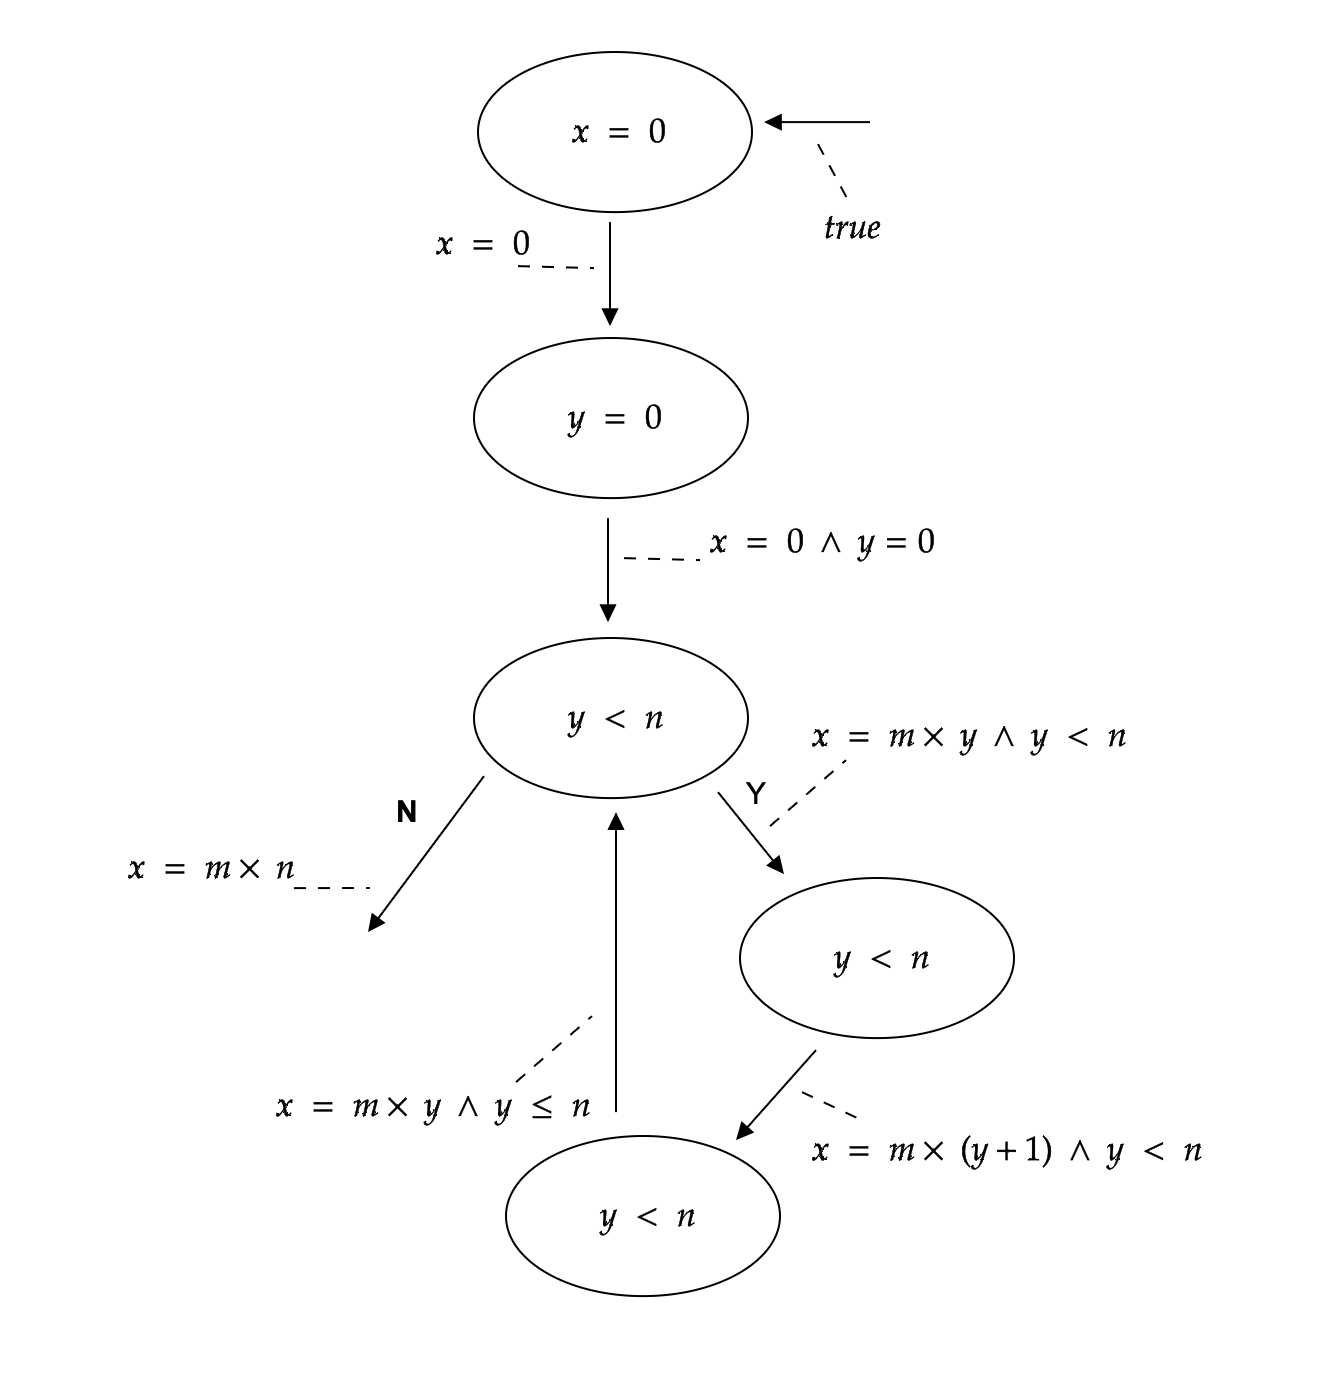
\includegraphics[width=\linewidth]{images/cf16.png}
%     \caption{Control flow graph of the program that computes $x = m * n$.}
%     \end{center}
%     \label{cf16}
% \end{figure*}

\begin{definition}[General Verification Conditions]
    In general, we can derive verification conditions using the following rules:
\begin{itemize}
    \item $\vc(\{\varphi\} ~\simp{{\sskip}}~ \{\psi\}) = \{\varphi \simplies \psi\}$.
    \item $\vc(\{\varphi\} ~\simp{x=a}~ \{\psi\}) = \{\varphi \simplies \psi[x \mapsto a]\}$.
    \item $\vc(\{\varphi\} ~\simp{c_1}~ \{\chi\} ~\simp{ c_2 }~ \{\psi\}) = \vc(\{\varphi\}~\simp{c_1}~ \{\chi\})\,  \cup \, \vc(\{\chi\} ~\simp{c_2}~ \{\psi\})$.
    \item $\vc(\{\varphi\} ~\sif{\simp{b}}{\simp{c_1}}{\simp{c_2}}~ \{\psi\}) = \vc(\{\varphi\land b\} ~\simp{c_1}~ \{\psi\}) \cup \vc(\{\varphi \land \neg b\}~\simp{c_2}~ \{\psi\})$.
    \item $\vc(\{\varphi\} \swhile{\simp{b}}{\simp{c}} \{\psi\}) = \{\varphi \simplies \chi, \chi \land \neg b \simplies \psi\} \cup \vc(\{\chi \land b\} ~\simp{c}~ \{\chi\})$.
\end{itemize}
\end{definition}



\subsection{Programs as predicate transforming (Dijkstra): Weakest (liberal) preconditions}

\begin{definition}[Weakest Liberal Preconditions] $\wlp(\simp{c}, \psi)$ is the \textit{weakest} $\varphi$ s.t $\{\varphi\} ~\simp{c}~ \{\psi\}$, i.e., for all $\varphi$ with $\{\varphi\} ~\simp{c}~\{\psi\}$ we have $ \varphi \simplies \wlp(\simp{c}, \psi)$.
\end{definition}

\begin{definition}[Weakest Preconditions] $\wsp(\simp{c}, \psi)$ is the \textit{weakest} $\varphi$ s.t $\{\varphi\} ~\simp{c}~ \{\psi\} \land \forall \sigma,$ if $\sigma \models \varphi$ then $\simp{c}$ terminates from $\sigma$.
\end{definition}

\begin{definition}
    An assertion language is \emph{expressive} if $\wlp(\simp{c},\psi) = \{\sigma \in \Sigma \mid \sop{c}{\sigma} = \bot \lor \forall \interp. \sde{c}{\sigma} \models_{\interp}\psi\}$.
\end{definition}

\begin{remark}
    For IMP, arithmetic $(\mathbb{N}, +, *)$ is expressive (proof by Goedelization of program executions).
\end{remark}


\begin{example} 
A few examples:
\begin{align*}
    \wlp(\sskip, \psi) &= \psi\\
    \wlp(\simp{x=a}, \psi) &= \psi[x\mapsto a]\\
    \wlp(\simp{c_1}, \simp{c_2}, \psi) &= \wlp(\simp{c_1}, \wlp(\simp{c_1}, \psi)) \\
    \wlp(\simp{\sif{b}{c_1}{c_2}}, \psi) &= (b\simplies \wlp(\simp{c_1}, \psi)) \land (\neg b \simplies \wlp(\simp{c_2}, \psi))\\
    &= (b \land \wlp(\simp{c_1}, \psi)) \lor (\neg b \land \wlp(\simp{c_2}, \psi)) \\
    \wlp(\simp{\swhile{b}{c}}, \psi)  &= \text{weakest} \; \chi:
    \chi \land b \simplies \wlp(\simp{c}, \chi) \land \chi \land \neg b \simplies \psi \\
    \wsp(\simp{\swhile{b}{c}}, \psi)  &= \text{weakest} \; \chi:
    \chi \land b \land (e=n) \simplies \wlp(\simp{c}, \chi\land e>n) \\
    &\quad\quad  \land \chi \land \neg b \simplies \psi \\
    &\quad \quad \land \chi\simplies  e \in \text{well-founded set}
\end{align*}
where $n$ is a fresh variable. 
    % \begin{itemize}
    %     \item $\wlp(\texttt{while } b \texttt{ do } c, \psi) = \texttt{weakest }\chi$ s.t 1) $\chi \land b \simplies \wlp(c, \chi)$ and 2) $\chi \land \neg b \simplies \psi$.
    %     \item For a fresh variable $n$, $\wsp(\texttt{while } b \texttt{ do } \simp{c}, \psi) = \texttt{weakest }\chi$ s.t for a fresh variable $n$ 1) $\chi \land b \land e = n \simplies \wlp(\simp{c}, \chi \land e > n)$, 2) $\chi \land \neg b \simplies \psi$, and 3) $\chi \simplies e \in $ well founded set.
    % \end{itemize}
\end{example}

